\clearpage
\section{Results}\label{res}
% JK: this section is trying to "set the stage" re. general epidemic conditions
%     for contextualizing subsequent results.
%     So, it's not specifically outlined in methods, but I think still useful to include?
Early epidemic emergence was driven by regular sex work partnerships
(Figures \ref{fig:inf.part}~and~\ref{fig:inf.alluvial}).
However, main/spousal partnerships contributed the majority of infections by 2000, % MAN (1997)
including 64\% (median) of new infections in 2020 in the base case. % MAN
By 2020, clients of FSW had transmitted the most infections (Figure~\ref{fig:inf.fr})
and lower risk women had acquired the most infections (Figure~\ref{fig:inf.to}).
Overall HIV prevalence in 2020 was median (95\% confidence interval):
\xci{bc/prev.all.2020}\% (Figure~\ref{fig:fit.prev}),
and overall incidence was \xci{bc/inc.all.2020} per 1000 person-years (Figure~\ref{fig:fit.inc}).
The prevalence ratio among FSW versus lower risk women was \xci{bc/pr.fsw.2020},
and among clients of FSW versus lower risk men it was \xci{bc/pr.cli.2020} (Figure~\ref{fig:fit.pr}).
Due to turnover and higher HIV incidence among FSW,
achieving similar rates of diagnosis among FSW versus other women (Figure~\ref{fig:fit.cas.dx})
required \xci{Rdx.fsw} times the rate of testing.
Sex work contributed a growing proportion of infections
over 2020--2040: from 21\% to 26\% (Figure~\ref{fig:inf.part}). % MAN
%===================================================================================================
\subsection{Influence of differences in cascade between risk groups}
Figure~\ref{fig:obj.1.inf.add} illustrates cumulative additional infections
in each counterfactual scenario (60-80-80 overall by 2020) versus the base case (95-95-95 overall by 2020);
Figure~\ref{fig:obj.1.inc.add} illustrates additional incidence.
Leaving behind FSW and clients resulted the most additional infections:
\xci{--/inf.add.2040}\% more than the base case by 2040.
By contrast, leaving behind neither FSW nor clients resulted in the fewest additional infections:
\xci{++/inf.add.2040}\% more than the base case by 2040 ---
a \xci{++/inf.add.vs.--.2040}\% reduction. % in additional infections.
Leaving behind either FSW or clients resulted in a similar number of additional infections:
\xci{+-/inf.add.2040}\% and \xci{-+/inf.add.2040}\%, respectively.
However, who acquired these additional infections differed (Figure~\ref{fig:inf.diff.to}),
with more additional infections among clients when FSW were left behind,
versus among lower risk risk women when clients were left behind.
The majority of additional infections were transmitted
via main/spousal partnerships in all scenarios (Figure~\ref{fig:inf.diff.part}).
\begin{figure}[h]
  \centering
  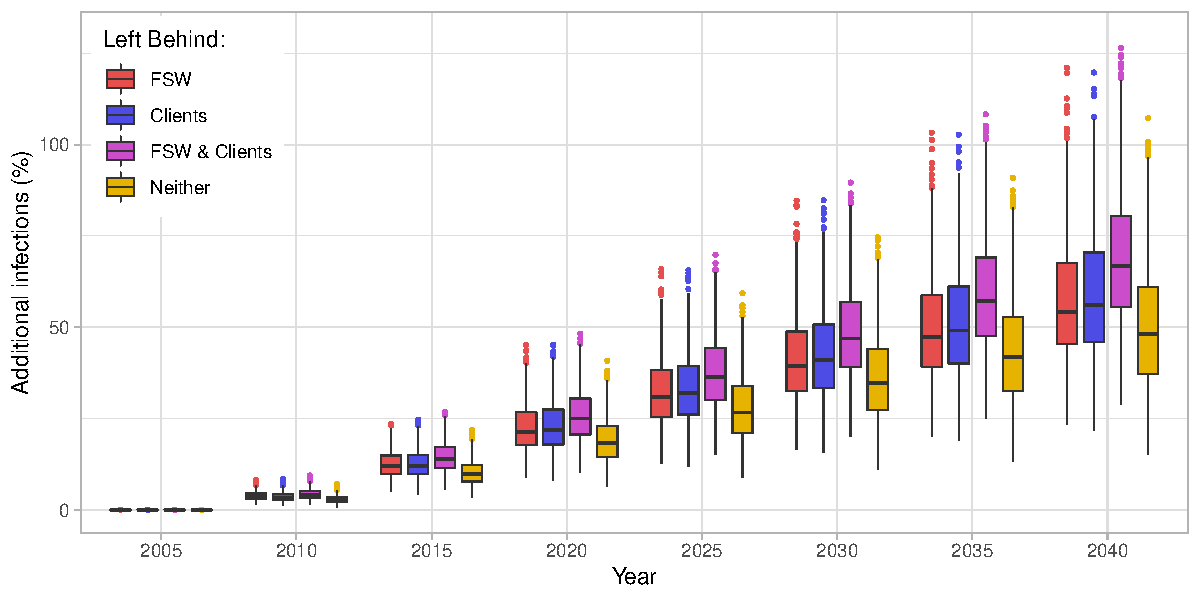
\includegraphics[width=\linewidth]{obj_1_inf_add}
  \caption{Cumulative additional HIV infections (\%) in counterfactual scenarios (60-80-80 overall by 2020)
    vs the base case scenario (95-95-95 by 2020).
    Scenarios explore reduced cascades (40-60-80 by 2020) among FSW, clients of FSW, both, or neither
    as part of reduced cascade overall.}
  \label{fig:obj.1.inf.add}
\end{figure}
%===================================================================================================
\subsection{Conditions under which cascade differences matter most}
Figure~\ref{fig:obj.2.inf} illustrates the standardized effects of
reduced viral suppression ($dVS$)
among FSW, clients, and the remaining population (``lower risk'')
on cumulative additional infections versus the base case by 2040,
as well as effect modification by epidemic conditions.
Trends were consistent across multiple time horizons (Figure~\ref{fig:obj.2.inf.t})
and for additional incidence by 2040 (Figure~\ref{fig:obj.2.inc}).
Reduced cascade among the lower risk population
had a larger independent effect than reduced cascade among FSW or clients,
likely due to larger group size and the highly generalized epidemic context.
Interaction between all pairs of $dVS$ terms were significant,
suggesting that reduced cascade across multiple sub-populations
synergistically contributes to additional infections,
perhaps reflecting residual transmission networks unreached by ART scale-up.
% JK: is this editorializing-ish? I'm trying to give a plainer-language re-statement of the result.
\begin{figure}
  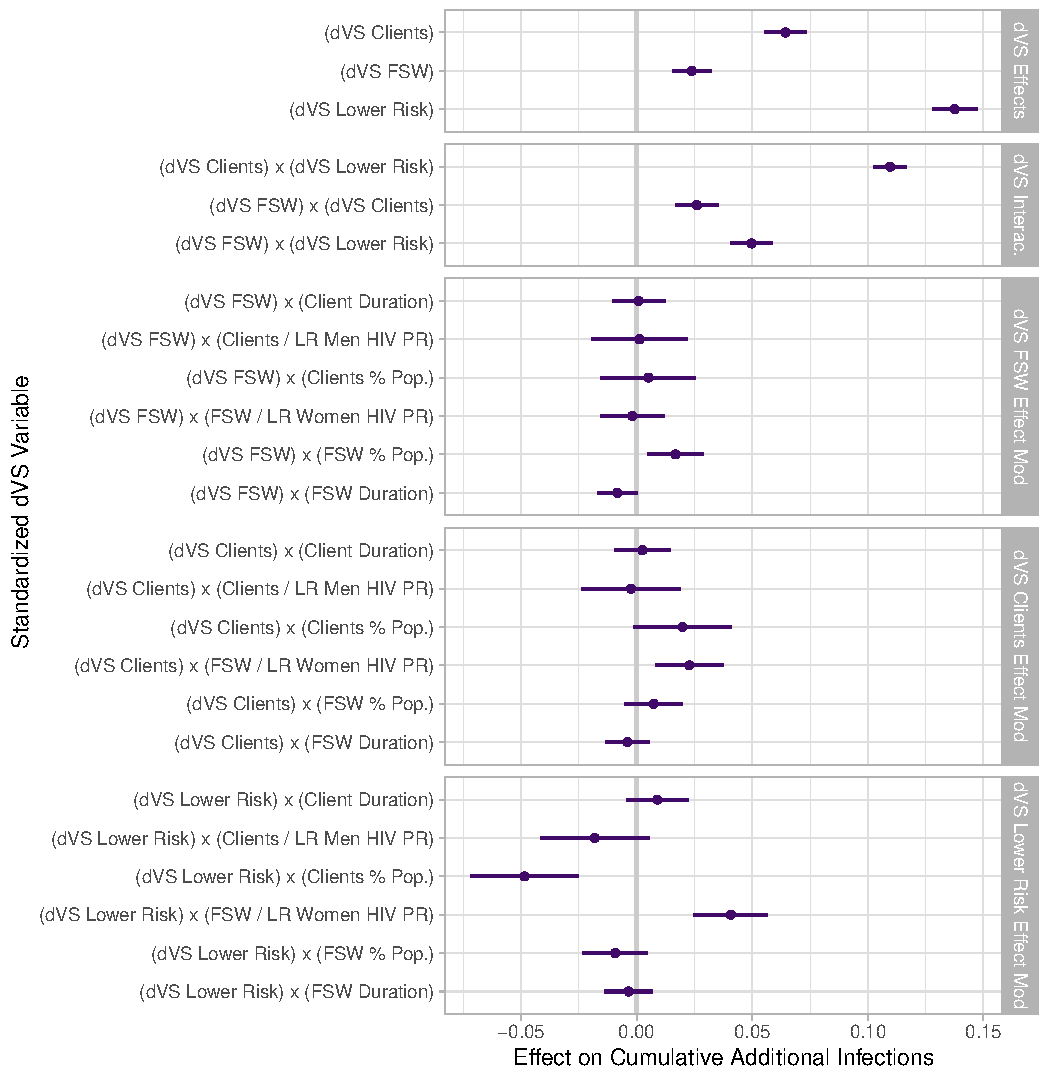
\includegraphics[width=\linewidth]{obj_2_inf}
  \caption{Standardized effects of reduced viral suppression (dVS) among different populations
    on cumulative additional infections by 2040,
    plus effect modification by epidemic conditions}
  \label{fig:obj.2.inf}
  \floatfoot{
    Points and lines show the mean and 95\% confidence interval for $\beta$ terms from Eq.~(\ref{eq:obj.2}).
    $dVS$: absolute difference in viral suppression in each counterfactual scenario versus the base case;
    FSW: female sex workers;
    Clients: of FSW;
    LR: lower risk;
    Duration: average time spent in the risk group;
    \% Pop: relative population size;
    HIV PR: HIV prevalence ratio.
    All model variables were standardized like
    $\hat{x}_k = (x_k - \mu_{x_k}) / \sigma_{x_k}$
    to reflect the relative influence of variables.}
\end{figure}
\par
% JK: @SM - maybe we can discuss further these results below after you review?
%     I'm still working to understand some mechanistically,
%     and have not added any hypothesis or explanation here or in discussion yet.
%     Especially why "FSW / lower risk women HIV prevalence ratio" acts as a positive effect modifier
%     for the impact of treating clients, and wider pop, but *not* of treating FSW themselves;
%     "positive" meaning: larger "FSW / lower risk prevalence ratio" ->
%     more additional infections when reduced VLS among that group
%     (or more infections averted by treating that group).
%     My hypothesis for clients is that FSW have the largest transmission impact *via* clients,
%     so that the actual # infections transmitted from FSW is modest (mainly to clients),
%     but the # infections transmitted from those infections (mainly by clients) is much larger.
%     For the wider pop though I really don't have many ideas...
%     Maybe something about turnover, but it would really only help explain if
%     many women entering sex work from lower risk are already living with HIV & achieved vls.
Reduced cascade among FSW was associated with more additional infections when
the FSW population size was larger, and when
the duration in sex work was shorter (marginal significance).
Reduced cascade among clients was associated with more additional infections when
the HIV prevalence ratio among FSW vs lower risk women was larger,
and when the client population size was larger (marginal significance).
Reduced cascade among lower risk men and women was associated with more additional infections when
the HIV prevalence ratio among FSW vs lower risk women was larger,
and when the client population size was smaller.